\documentclass[12pt]{article}
% Layout
\usepackage[a4paper, portrait, margin=1in]{geometry}
\usepackage[none]{hyphenat}
\usepackage{titling}
% Math
\usepackage{amsmath}
\usepackage{amssymb}
\usepackage{mathtools}
\usepackage{mathrsfs}
\DeclareMathOperator{\sinc}{sinc}
\DeclareMathOperator{\rect}{rect}
% Captions
\usepackage[format=plain,
    font={small, it}, justification=centering]{caption}
\usepackage{subcaption}
\usepackage{hyperref}
\usepackage{cleveref}
\hypersetup{
    colorlinks,
    linkcolor={red!50!black},
    citecolor={blue!50!black},
    urlcolor={blue!80!black}
}
\usepackage{parskip}
\setlength\parindent{0pt}

% Itemize & enumerate
\usepackage{enumitem}

% Numbering of sections
\renewcommand{\thesubsection}{\thesection.\arabic{subsection}.}
\renewcommand{\thesubsubsection}{\roman{subsubsection}.}

% MATLAB CODE
\usepackage{minted}
\setminted{frame=single, obeytabs=true, tabsize=4, breaklines=true, numbersep = -12pt, linenos=true, fontsize=\scriptsize}
\usemintedstyle{vs}
% Data Visualisation
\usepackage{pgfplots}
\pgfplotsset{width=10cm, compat=1.18}
\usepackage{tikz}
\usetikzlibrary{patterns}
\usepackage{graphicx}
\usepackage{wrapfig}
\usepackage{tabularx}
\setkeys{Gin}{width=14cm}
\newcolumntype{Y}{>{\centering\arraybackslash}X}
\pgfdeclarepatternformonly{nelw}%
{\pgfqpoint{-1pt}{-1pt}}%
{\pgfqpoint{10pt}{10pt}}%
{\pgfqpoint{9pt}{9pt}}%
{
    \pgfsetlinewidth{0.4pt}
    \pgfpathmoveto{\pgfqpoint{0pt}{0pt}}
    \pgfpathlineto{\pgfqpoint{9.1pt}{9.1pt}}
    \pgfusepath{stroke}
}
\usetikzlibrary{external}
\tikzexternalize[prefix=figures/]
% Itemize & enumerate
\usepackage{enumitem}

% Numbering of sections
\renewcommand{\thesubsection}{\thesection.\arabic{subsection}}
\renewcommand{\thesubsubsection}{\roman{subsubsection}.}

% Numbering of items
\numberwithin{equation}{section}
\numberwithin{figure}{section}
\numberwithin{table}{section}
\renewcommand{\refname}{}
% FROM EXAMPLE ASS - EGB242
\newcommand{\horrule}[1]{\rule{\linewidth}{#1}}
% METADATA
\author{
    Charlie Turner \small n10752846 \and
    Joel Kemp \small n10746862 \and
    Viet Truong Minh \small n10440151
}
\title{
    \normalfont{} \normalsize{}
    \begin{flushleft}
        \textsc{Queensland University of Technology, EGB242} \\ [5pt]
    \end{flushleft}
    \horrule{0.5pt} \\[0.4cm]
    \huge Assignment 2 \\
    \large \textsc{MARS242 --- Orbiting The Red Planet}   \\ % The assignment title
    \horrule{2pt} \\[0.2cm]
    \textbf{Group 14} \\
}

\begin{document}

\begin{titlingpage}
    \maketitle
\end{titlingpage}

\section*{Introduction}

After the chief at Brisbane-based Australian Space Agency (BASA) has reviewed
previous tasks, they have decided to assign the team `live' supervision of the
MARS-242 mission.

Communication between the ground and the mission must be clear and
uninterrupted to ensure the mission is safe and smooth. There are three
important tasks to be completed:
\begin{itemize}
    \item[-] Identifying an appropriate landing site for the crew
    \item[-] Ensuring the safety of the Martian habitats for the current and future crews
\end{itemize}

To achieve these objectives, the team must be able to properly interpret and
analyse data streams from a rover scouting the surface prior to landing. The
landing site must be identified despite periodic and bandlimited noise
disrupting signal streams. Once a landing site is determined, the acoustic
properties of the habitat's rooms must be analysed, removing interference and
noise arising from the communication channel and method.

%--------------------------------------------------------------------------
%
% SECTION 1: MARS ROVER
%
%--------------------------------------------------------------------------
\section{Mars Rover}

With the crew landing soon, a rover has been gathering data regarding possible
landing sites. Until a malfunction on the rover, data has been communicated
directly with Earth, where it can be analysed and the results sent directly to
astronauts on board Mars-242. The rover's data is vital for the survival of the
mission, so a solution has been found to send the raw data directly to
astronauts.

\subsection{Communication Channels}
The spaceship's communication channel consists of a constant-magnitude function
in the frequency domain, between $-7100$Hz and $+7100$Hz with some magnitude
$A$. This can be represented by the rectangular function
\begin{equation*}
    C_{ship}(f) = A \rect{\frac{f}{14200}}
\end{equation*}
and the magnitude spectrum represented in Fig.~\ref{fig:p1-ship}.
\begin{figure}[ht]
    \centering
    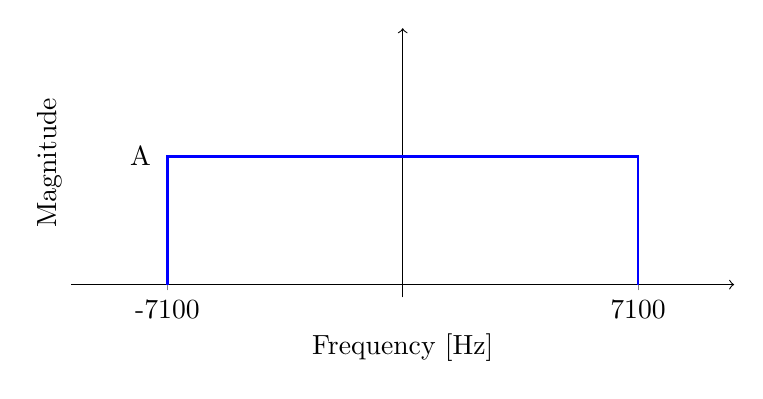
\begin{tikzpicture}
        \begin{axis}[
                width=10cm , height=5cm,
                ymin=-0.1, ymax=2,
                xmin=-10000, xmax=10000,
                axis lines = middle,
                axis line style={->},
                x label style={at={(axis description cs:0.5,-0.1)},anchor=north},
                y label style={at={(axis description cs:-0,.5)},rotate=90,anchor=south},
                ylabel = Magnitude,
                xlabel = {Frequency [Hz]},
                xtick ={-7100, 0, 7100 },
                xticklabels = {-7100, 0, 7100},
                ytick = {0, 1},
                yticklabels = {, A},
                yticklabel style = { xshift=-3cm},
                scaled ticks = false
            ] \addplot[ color = blue, line width = 1pt, ] coordinates {(-7100, 0) (-7100, 1) (7100, 1) (7100, 0)};
        \end{axis}
    \end{tikzpicture}
    \caption{Frequency Spectrum of the ship's communication channel\label{fig:p1-ship}}
\end{figure}

\subsection{Rover Transmission Function}
The rover's transmission function is known as a function of time, given by:
\begin{equation*}
    s_{rov}(t) = 8000 \times \sinc^2(4000t)\cos(2\pi \times 8000t)
\end{equation*}
Using the property of duality, the fourier transform of this function can be
calculated, noting that the Fourier transform of the $\sinc^2$ function is the
triangular function:
\begin{equation*}
    \triangle_T(t) \xleftrightarrow{\mathscr{F}} T\sinc^2(Tf)
\end{equation*}
Since the triangular function is an even function, it is also known that
$\triangle_T(-f) = \triangle_T(f)$. From prior tasks the team has determined
that a multiplication by a cosine term in the time domain results in a Frequency
modulation, so the Fourier Transform of the rover's transmission function can be
calculated as:
\begin{align*}
    4000 \sinc^2(4000t)   & \xrightarrow{\mathscr{F}} \triangle_{4000}(f)                                           \\
    \therefore S_{rov}(f) & = 2 \times \frac{1}{2} \bigg[ \triangle_{4000}(f-8000) + \triangle_{4000}(f+8000)\bigg] \\
                          & = \triangle_{4000}(f-8000) + \triangle_{4000}(f+8000)
\end{align*}

Plotting this function in Fig.~\ref{fig:p1-rov}, we can see that the rover's
transmission function takes the form of a triangular function with bandwidth of
$4000$, modulated to both positive and negative $8000$Hz:

\begin{figure}[ht]
    \centering
    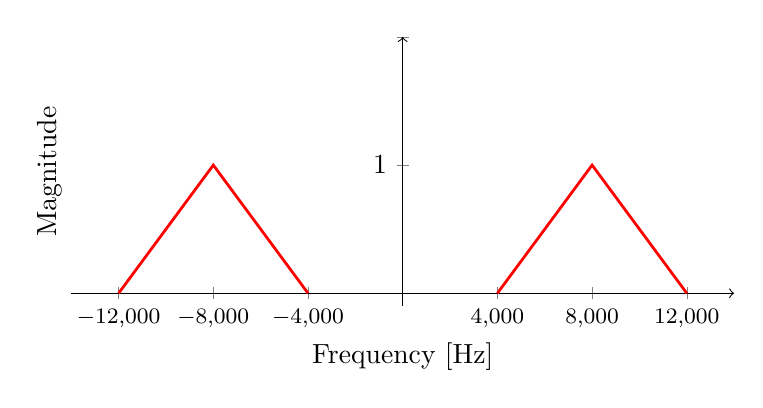
\begin{tikzpicture}
        \begin{axis}[
                width=10cm , height=5cm,
                ymin=-0.1, ymax=2,
                xmin=-14000, xmax=14000,
                axis lines = middle,
                axis line style={->},
                x label style={at={(axis description cs:0.5,-0.1)},anchor=north},
                y label style={at={(axis description cs:-0,.5)},rotate=90,anchor=south},
                ylabel = Magnitude,
                xlabel = {Frequency [Hz]},
                xtick = {-12000, -8000, -4000, 0, 4000, 8000, 12000},
                ytick = {0, 1, 2},
                yticklabels = {, 1, },
                x tick label style={font=\footnotesize},
                scaled ticks = false
            ]
            \addplot[color = red, line width = 1pt] coordinates {(-12000, 0) (-8000, 1) (-4000, 0)};
            \addplot[color = red, line width = 1pt] coordinates {(4000, 0) (8000, 1) (12000, 0)};
        \end{axis}
    \end{tikzpicture}
    \caption{Rover Transmission Function\label{fig:p1-rov}}
\end{figure}

\pagebreak
\subsection{Filter Broadcast Information}
To ensure the rover's signal is recieved fully, a filter must be applied to the
data broadcasted by the ship. As the ship broadcasts on $7100$Hz unmodulated
band, a high-pass filter is ideal. To design the filter, the frequency domain
of both the ship's and rover's communication channels was sketched
(Fig.~\ref{fig:p1-channels}).

\begin{figure}[ht]
    \centering
    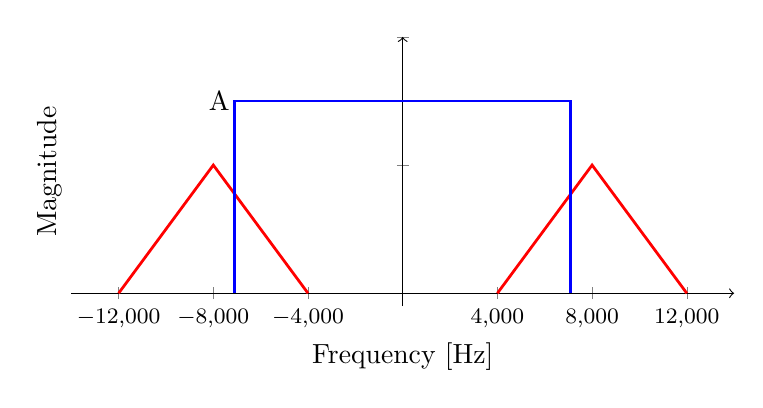
\begin{tikzpicture}
        \begin{axis}[
                width=10cm , height=5cm,
                ymin=-0.1, ymax=2,
                xmin=-14000, xmax=14000,
                axis lines = middle,
                axis line style={->},
                x label style={at={(axis description cs:0.5,-0.1)},anchor=north},
                y label style={at={(axis description cs:-0,.5)},rotate=90,anchor=south},
                ylabel = Magnitude,
                xlabel = {Frequency [Hz]},
                xtick = {-12000, -8000, -4000, 0, 4000, 8000, 12000},
                ytick = {0, 1, 1.5, 2},
                yticklabels = {, , A, },
                yticklabel style = { xshift=-2cm},
                x tick label style={font=\footnotesize},
                scaled ticks = false
            ]
            \addplot[color = red, line width = 1pt] coordinates {(-12000, 0) (-8000, 1) (-4000, 0)};
            \addplot[color = red, line width = 1pt] coordinates {(4000, 0) (8000, 1) (12000, 0)};
            \addplot[ color = blue, line width = 1pt, ] coordinates {(-7100, 0) (-7100, 1.5) (7100, 1.5) (7100, 0)};
        \end{axis}
    \end{tikzpicture}
    \caption{Combined communication channels\label{fig:p1-channels}}
\end{figure}

The cut-off frequency must be chosen so that it does not disrupt the incoming
signal from the rover, but fully removes the noise from the ship's
communication channel. As the rover's signal has been modulated to $8000$Hz, as
long as we preserve a full half of it's triangular frequency channel no
information loss will occur. $8000$Hz has been chosen as the cut-off frequency,
as it will ensure that these requirements are met. The transfer function is
then:
\begin{equation*}
    |H(f)| = \begin{cases}
        1, |f| > 8000 \\
        0, |f| < 8000
    \end{cases}
\end{equation*}

As can be seen in Fig.~\ref{fig:p1-filter}, this is the most simplistic ideal
filter for the task, and when applied in the frequency domain will either leave
a frequency component as it is, or remove it entirely.

\begin{figure}[ht]
    \centering
    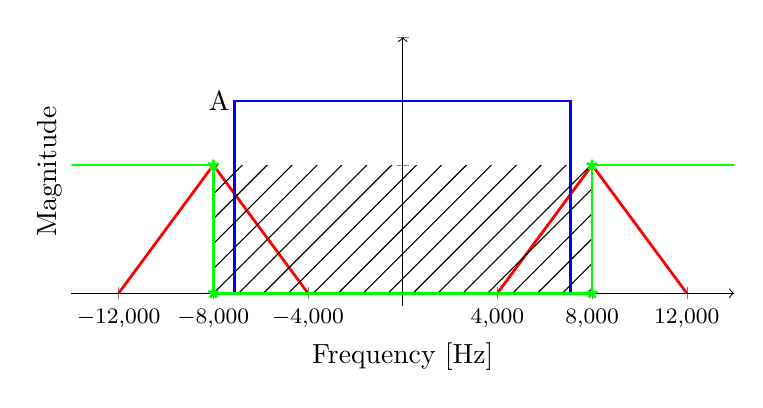
\begin{tikzpicture}
        \begin{axis}[
                width=10cm , height=5cm,
                ymin=-0.1, ymax=2,
                xmin=-14000, xmax=14000,
                axis lines = middle,
                axis line style={->},
                x label style={at={(axis description cs:0.5,-0.1)},anchor=north},
                y label style={at={(axis description cs:-0,.5)},rotate=90,anchor=south},
                ylabel = Magnitude,
                xlabel = {Frequency [Hz]},
                xtick = {-12000, -8000, -4000, 0, 4000, 8000, 12000},
                ytick = {0, 1, 1.5, 2},
                yticklabels = {, , A, },
                yticklabel style = { xshift=-2cm},
                x tick label style={font=\footnotesize},
                scaled ticks = false
            ]
            \addplot[color = red, line width = 1pt] coordinates {(-12000, 0) (-8000, 1) (-4000, 0)};
            \addplot[color = red, line width = 1pt] coordinates {(4000, 0) (8000, 1) (12000, 0)};
            \addplot[ color = blue, line width = 1pt, ] coordinates {(-7100, 0) (-7100, 1.5) (7100, 1.5) (7100, 0)};
            \addplot+[color = green, line width = 1pt, pattern=nelw] coordinates {(-20000, 1) (-8000, 1) (-8000, 0) (8000, 0) (8000, 1) (20000, 1)};
        \end{axis}
    \end{tikzpicture}
    \caption{High-pass filter visualisation process\label{fig:p1-filter}}
\end{figure}

Graphically, we can see that the resulting signal will have none of the ship's
broadcast frequencies, and only the outer half of the triangular rover
transmission signal mirrored in the positive and negative frequencies.
\pagebreak
\subsection{Signal Recovery}
To recover the filtered signal described in the previous section, we can use
the modulation property once again to recover the signal. Since the function
was modulated to $\pm 8000$Hz, we can recover it back to $0$Hz by multiplying
by $\cos(2\pi 8000t)$ in the time domain. In the frequency domain this is
easily visualised, and the demodulated signal is represented in
Fig.~\ref{fig:p1-demod}.

\begin{figure}[ht]
    \centering
    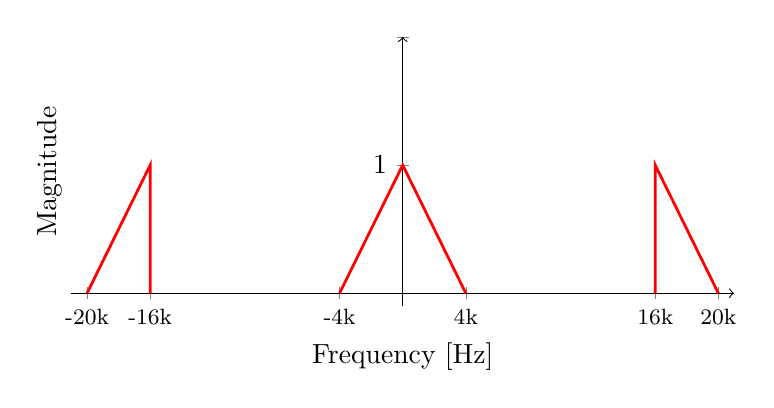
\begin{tikzpicture}
        \begin{axis}[
                width=10cm , height=5cm,
                ymin=-0.1, ymax=2,
                xmin=-21000, xmax=21000,
                axis lines = middle,
                axis line style={->},
                x label style={at={(axis description cs:0.5,-0.1)},anchor=north},
                y label style={at={(axis description cs:-0,.5)},rotate=90,anchor=south},
                ylabel = Magnitude,
                xlabel = {Frequency [Hz]},
                xtick = {-20000, -16000, -4000, 0, 4000, 16000, 20000},
                xticklabels = {-20k, -16k, -4k, 0, 4k, 16k, 20k},
                ytick = {0, 1, 2},
                yticklabels = {, 1,  },
                x tick label style={font=\footnotesize},
                scaled ticks = false
            ]
            \addplot[color = red, line width = 1pt] coordinates {(-20000, 0) (-16000, 1) (-16000, 0)};
            \addplot[color = red, line width = 1pt] coordinates {(-4000, 0) (0, 1) (4000, 0)};
            \addplot[color = red, line width = 1pt] coordinates {(16000, 0) (16000, 1) (20000, 0)};
        \end{axis}
    \end{tikzpicture}
    \caption{Demodulated Rover Signal\label{fig:p1-demod}}
\end{figure}

To remove the high frequency copies of the signal left behind, we can once
again use an ideal filter. This time, a low-pass filter is used, and the cutoff
frequency is chosen to be $4000$Hz. $4000$Hz is chosen as it guarantees that
any noise outside of the rover's frequency channel will be removed. The
transfer function for this filter is therefore:

\begin{equation*}
    |H(f)| = \begin{cases}
        1, |f| < 4000 \\
        0, |f| > 4000
    \end{cases}
\end{equation*}

Multiplying the filter transfer function and the demodulated signal in the
frequency domain, the resulting frequency domain of the rover's signal shown in
Fig.~\ref{fig:p1-filter-demod}.

\begin{figure}[ht]
    \centering
    \begin{tikzpicture}
        \begin{axis}[
                width=10cm , height=5cm,
                ymin=-0.1, ymax=2,
                xmin=-21000, xmax=21000,
                axis lines = middle,
                axis line style={->},
                x label style={at={(axis description cs:0.5,-0.1)},anchor=north},
                y label style={at={(axis description cs:-0,.5)},rotate=90,anchor=south},
                ylabel = Magnitude,
                xlabel = {Frequency [Hz]},
                xtick = {-20000, -16000, -4000, 0, 4000, 16000, 20000},
                xticklabels = {-20k, -16k, -4k, 0, 4k, 16k, 20k},
                ytick = {0, 1, 2},
                yticklabels = {, 1,  },
                x tick label style={font=\footnotesize},
                scaled ticks = false
            ]
            \addplot[color = red, line width = 1pt] coordinates {(-4000, 0) (0, 1) (4000, 0)};
        \end{axis}
    \end{tikzpicture}
    \caption{Final frequency domain of rover's signal\label{fig:p1-filter-demod}}
\end{figure}

Despite multiple filtering stages, no information is lost from this process.
This can be justified with the knowledge that the negative frequency domain of
the Fourier Transform is a mirror of the positive domain. This means that the
modulation term ($\cos(2\pi 8000t)$) in the rover's transmission signal
effectively results in each half of the triangular frequency band containing
the same information. As we filtered only one half of this signal before
demodulating, the resulting signal can be guaranteed to contain the entirety of
information transmitted by the rover.

\subsection{Practical Filter Considerations}
In a more practical circumstance, information may end up being lost due to the
nature of practical analogue filters. However, since the shape of our frequency
spectrum is a triangle, cut-off frequencies may be determined so that only a
small amount of information would be lost and shouldn't impact the signal too
much. The inability to construct an analogue filter with instant roll-off also
means that noise would very likely persist from the ship's broadcast channel.
To mitigate this as much as possible, the filter used in the high-pass stage
should be of the highest order feasible for the application, which will have
the steepest frequency response. Increasing the cut-off frequency of the low
pass filter will also mitigate information loss, as long as the high frequency
copies are still attenuated sufficiently. \pagebreak

%--------------------------------------------------------------------------
%
% ---------------------SECTION 2: LANDING SITE-----------------------------
%
%--------------------------------------------------------------------------
\section{Choosing a Landing Site}

The surface-based rover has collected and transmitted images of possible
landing sites. Unfortunately, the transmission encountered both periodic and
bandlimited noise, so the signals must be denoised to observe the intended
images. One of the noisy images is visualised in Fig.~\ref{fig:p2-noisy}. This
is achieved in MATLAB using the \verb+reshape+ function, reshaping the incoming
1D data stream into a matrix, knowing that the images are all of the same size
(640$\times$480).

\begin{figure}[ht]
    \centering
    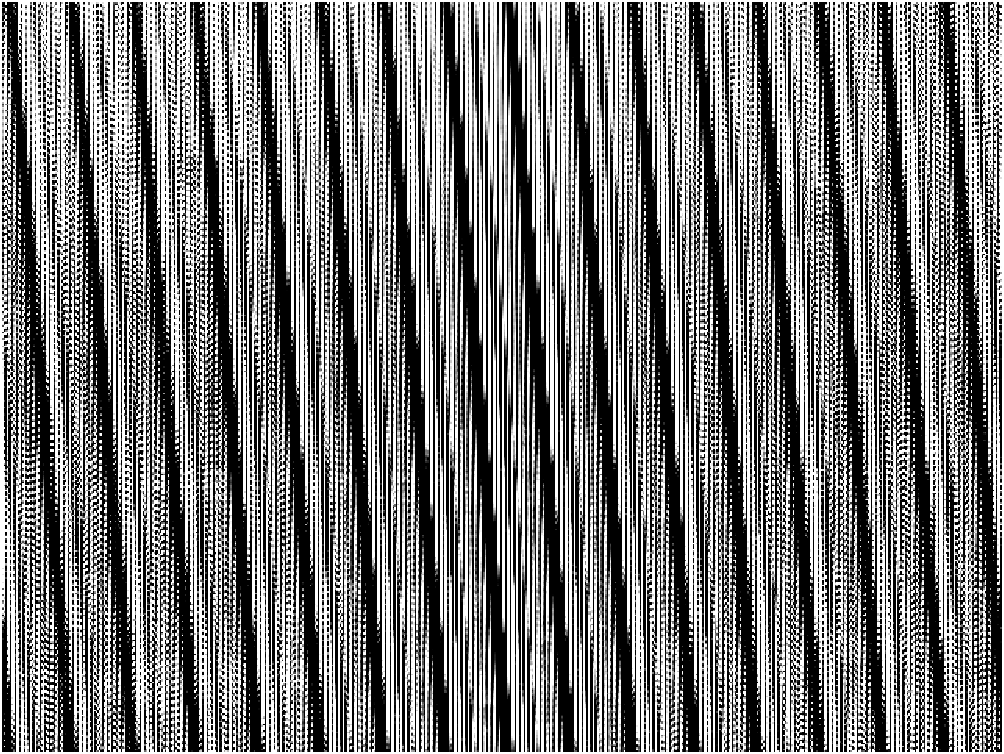
\includegraphics[width=7cm]{figures/p2-noisy.png}
    \caption{Noisy image of possible landing site\label{fig:p2-noisy}}
\end{figure}

\subsection{Modelling Periodic Noise}

To understand the characteristics of relevant noise, the signal is plotted in
both the time and frequency domain as in Fig.~\ref{fig:p2-timefreq},
understanding the importance of the sampling rate for the incoming signal:
\begin{minted}{matlab}
    Fs = 1000;                                              % Pixel Sampling Rate [Hz]
    T = pixels/Fs;                                          % Time to recieve an image
    t = linspace(0, T, length(sig)+1);                      % Time vector for full image
    f = linspace(-Fs/2, Fs/2, length(sig)+1);               % Frequency Vector
\end{minted}

\begin{figure}[h]
    \centering
    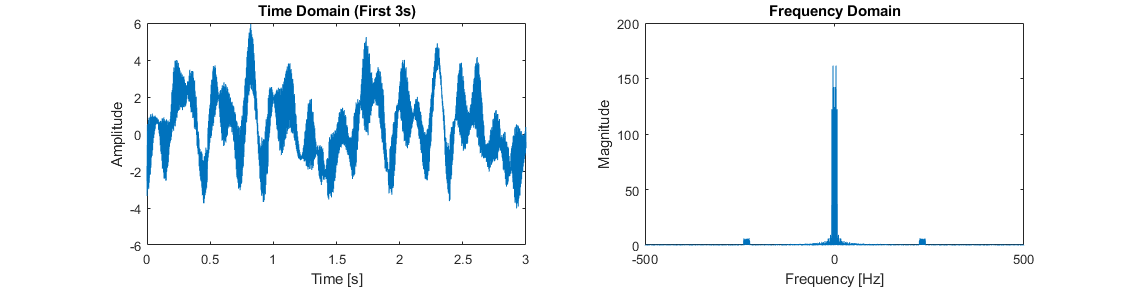
\includegraphics{figures/p2-timefreq.png}
    \caption{Time and Frequency Domain of Incoming Signal\label{fig:p2-timefreq}}
\end{figure}

While the full signal for an image is over 300 seconds long, plotting only the
first three seconds shows that there is a significant periodic noise present in
the time domain. Engineers at mission control have identified a set of possible
periods for the noise, and graphically we can determine that it appears to be
approximately 1.477 seconds long, confirming the engineers approximations.
Using MATLAB and the provided \verb+estimateNoise+ function, a vector
representing one period of this noise was computed:
\begin{minted}[firstnumber=61]{matlab}
    T = candidateT(1);                                      % period of noise
    periodInSamples = T * Fs;                               % samples in noise period
    Noisesig = estimateNoise(sig(1, :), periodInSamples);   % estimated noise function
\end{minted}

Comparing the estimated noise to the received signal in
Fig.~\ref{fig:p2-noisecomp}, we can see that the overall shape of the signals
is similar.

\begin{figure}[ht]
    \centering
    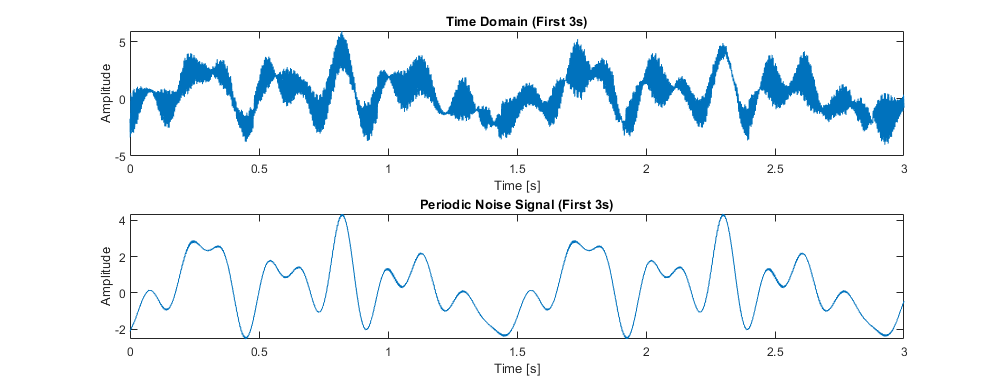
\includegraphics{figures/p2-noisecomp.png}
    \caption{Comparison of Estimated Noise and Recieved Signal\label{fig:p2-noisecomp}}
\end{figure}

With the correct discrete representation of periodic noise determined, we can
model \verb+Noisesig+ with a complex fourier series as follows:

\begin{align*}
    x(t)             & = \sum_{n=-\infty}^{\infty} c_n e^{j 2\pi n f_0 t}          \\
    \text{with } c_n & = \frac{1}{T} \int^{t_0 + T}_{t_0} x(t)e^{-j2\pi nf_0 t} dt
\end{align*}

In MATLAB, integrals are substituted for Riemann sums on the discrete vector,
computing $c_n$ for $-6\le n \le 6$ taking into account an accurate time vector
and sampling rate:

\begin{minted}[firstnumber=79]{matlab}
    t1= t(t<T); t1(end) = [];                               % Noise Time vector 
    ts = t1(2)-t1(1);                                       % Sampling interval [s]
    f0 = 1/T;                                               % Fundamental Frequency
    N = 6;                                                  % Number of harmonics
    n = (-N:N).';                                           % Vector of harmonics
    cn = f0 * Noisesig * exp(-1j*2*pi*f0*n*t1).' * ts;      % Fourier coefficients
    c0 = cn(N+1);                                           % DC coefficient
\end{minted}

The DC coefficient is computed as $c_0 = +0.3571$, and the complex coefficients
for the first 6 harmonics as follows:
\[
    \begin{array}{ccc}
        c_{-6} : -0.2208 + 0.4813i & c_{-5} : +0.2479 - 0.2237i & c_{-4} : +0.0260 - 0.1276i \\
        c_{-3} : -0.4525 + 0.1048i & c_{-2} : -0.2916 + 0.2814i & c_{-1} : -0.3702 + 0.1522i \\
        c_{+1} : -0.3702 - 0.1522i & c_{+2} : -0.2916 - 0.2814i & c_{+3} : -0.4525 - 0.1048i \\
        c_{+4} : +0.0260 + 0.1276i & c_{+5} : +0.2479 + 0.2237i & c_{+6} : +0.2208 + 0.4813i \\
    \end{array}
\]

BASA has confirmed that there should be no DC component to the periodic noise.
Because $c_0$ represents the DC component of the Fourier series, this term can
simply be equated to 0 in order to remove this bias:

\begin{minted}[firstnumber=90]{matlab}
    c0 = 0;                                                 % DC coefficient
    cn(N+1) = c0;                                           % Corresponding coefficient in cn vector 
\end{minted}

With the correct Fourier coefficients determined, the signal can be
reconstructed for the total period of the image signal, as per the following:
\begin{minted}[firstnumber=93]{matlab}
    Noisesig_fs = cn * exp(1j*2*pi*f0*n*t);                 % Fourier series for total t
\end{minted}

To test the accuracy of the model, this Fourier approximation was plotted
against the estimated noise profile for one period, as seen in
Fig.~\ref{fig:p2-noisefscomp}:

\begin{figure}[h]
    \centering
    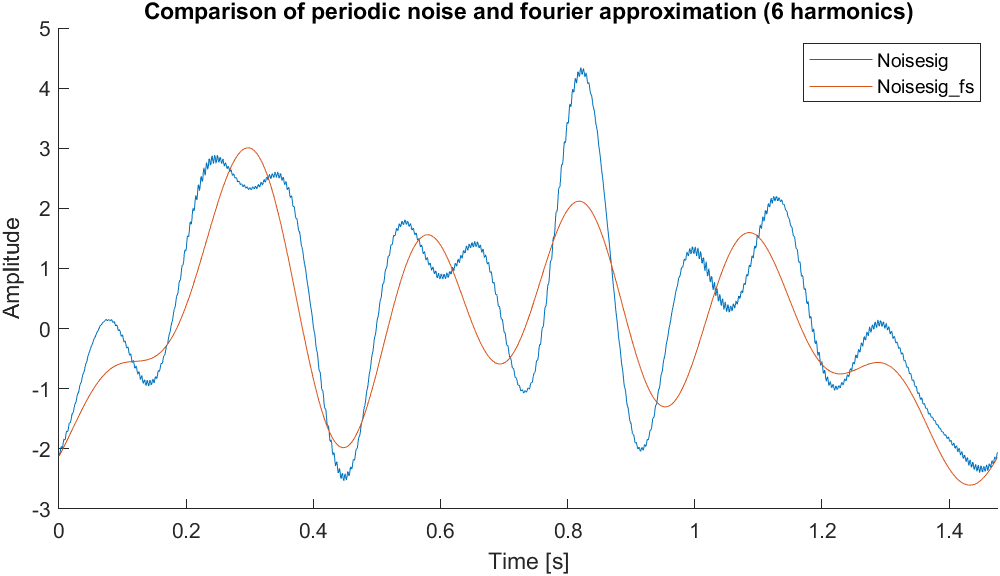
\includegraphics[width=9cm]{figures/p2-noisefscomp.png}
    \caption{Estimated noise and Fourier series approximation\label{fig:p2-noisefscomp}}
\end{figure}

Visually, the Fourier approximation using 6 harmonics does not provide a full
representation of the signal, as it is unable to model the more detailed noise
at the peaks and such. The overall shape of the noise is represented, but it is
expected that the denoising may not be sufficient for recoving detail within
the image.
\subsection{Removing Periodic Noise}
The above period noise approximation can be tested by subtracting the periodic
noise from the incoming image signal:

\begin{minted}[firstnumber=130]{matlab}
    im1(1,:) = sig(1,:) - Noisesig_fs;                      % First image with periodic noise removed
\end{minted}

As with the original signal, this denoised signal was then reshaped and shown
in Fig.~\ref{fig:p2-im1}, along with the frequency domain representation:

\begin{figure}[ht]
    \centering
    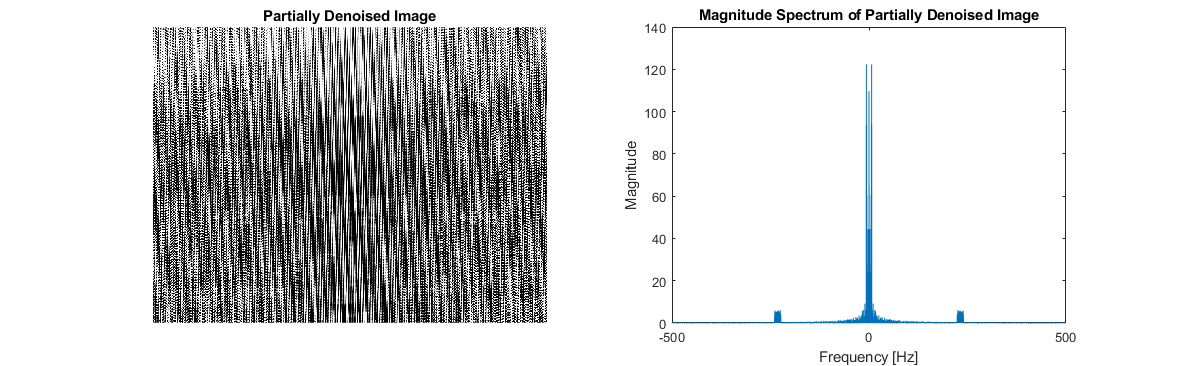
\includegraphics{figures/p2-im1.png}
    \caption{Image and Magnitude Spectrum with periodic noise removed\label{fig:p2-im1}}
\end{figure}

As expected, the image is not noticeably clearer than the original, with strong
lines still obscuring the intended picture. The magnitude spectrum confirms
this noise, with large frequency spikes present at specific low frequencies.
This indicates that there is still considerable periodic noise present. To
improve the noise approximation, a more suitable number of harmonics would be
10, as it captures the details much more accurately. It also requires very
little extra computational power, taking only about 0.03 seconds longer to
compute the Fourier approximation. The effect of 10 harmonics is shown in
Fig.~\ref{fig:p2-compharms}:

\begin{figure}[ht]
    \centering
    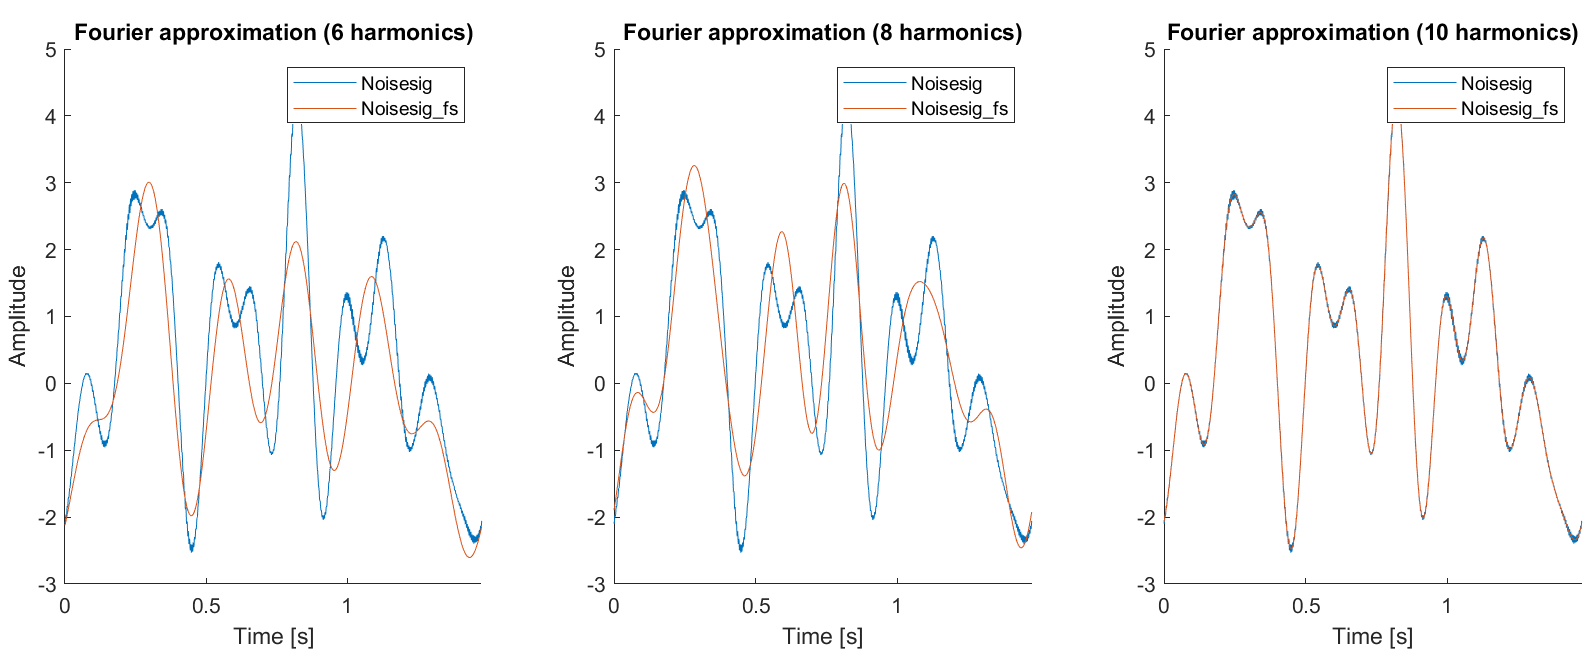
\includegraphics{figures/p2-compharms.png}
    \caption{Comparison of fourier series (6, 8, and 10 harmonics)\label{fig:p2-compharms}}
\end{figure}

Now with 10 harmonics to better approximate the periodic noise, we can once
again denoise the image, shown in Fig.~\ref{fig:p2-im1improved}:

\begin{figure}[ht]
    \centering
    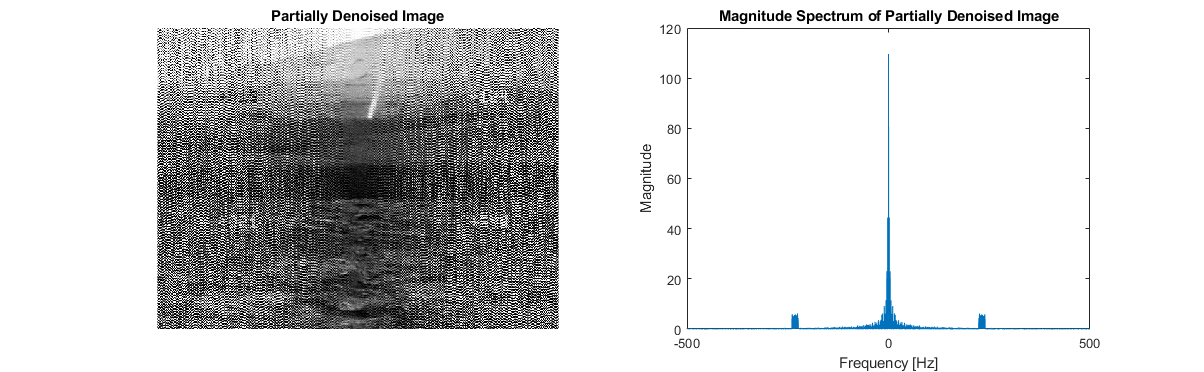
\includegraphics{figures/p2-im1improved.png}
    \caption{Improved Denoised Image and Magnitude Spectrum\label{fig:p2-im1improved}}
\end{figure}

The strong predictable lines corrupting the image are now much less pronounced,
and the outline of what resembles a mountain and rocky terrain can be
distinguished. However, the image is still much too noisy to discern the
specific location. \pagebreak
\subsection{Removing Bandlimited Noise}

\begin{wrapfigure}{r}{0.4\textwidth}
    \vspace*{-12pt}
    \centering
    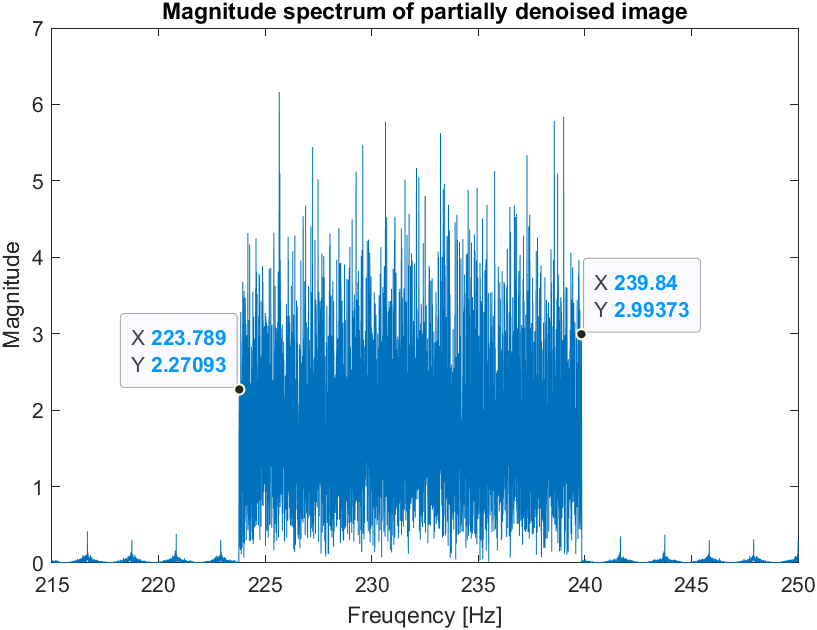
\includegraphics[width=6cm]{figures/p2-bandnoise.png}
    \caption{Magnitude spectrum of bandlimited noise\label{fig:p2-bandnoise}}
\end{wrapfigure}

The frequency band for bandlimited noise was determined visually as in
Fig.~\ref{fig:p2-bandnoise}, with a lower limit of $\pm 223$Hz, and upper limit
of $\pm 240$Hz. A band stop filter was created to remove the noise. This is
achieved in MATLAB in the frequency domain, which is much more easy to
visualise. The filter was constructed as a vector corresponding to the full
frequency vector, multiplying frequency components within the band by zero,
while leaving other data untouched. Finally, the inverse Fourier transform must
be computed to convert the de-noised signal back to the time domain for
viewing:
\begin{minted}[firstnumber=150]{matlab}
    B_low = 223;                                                % Lower bandwidth frequency
    B_high = 240;                                               % Upper bandwidth frequency
    filter = ones(size(f));                                     % Initiallise with ones
    filter((abs(f) > B_low) & (abs(f) < B_high)) = 0;           % Assign 0 to elements in band
    filtered = fftshift(IM1(1,:)) .* filter;                    % Filter in frequency domain
    im2 = zeros(size(sig));                                     % Initialise for performance
    im2(1,:) = ifft(ifftshift(filtered));                       % Filtered image signal in time domain
\end{minted}

Showing this final image in Fig.~\ref{fig:p2-im1recov}, we can see that the
picture has been recovered, including the navigational numbers which were not
visible after removing only the periodic noise:

\begin{figure}[ht]
    \centering
    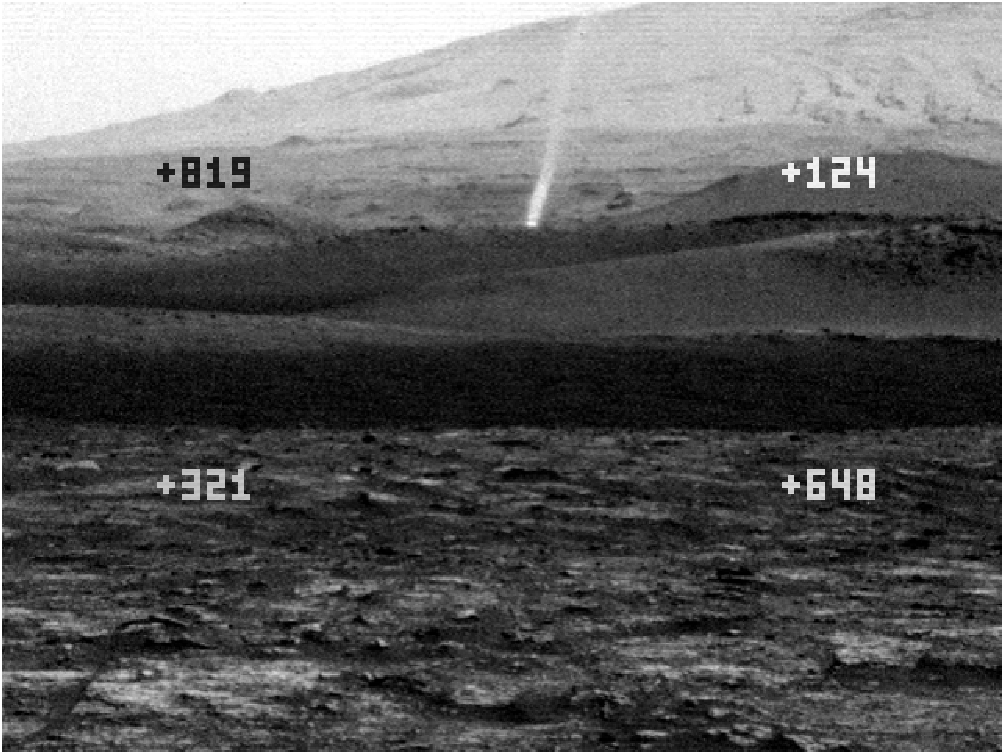
\includegraphics[width=9cm]{figures/p2-im1recov.png}
    \caption{Recovered image from the rover\label{fig:p2-im1recov}}
\end{figure}

\pagebreak
\subsection{Choosing A Site}
The removal of periodic noise was done as above for all four images, however
removing bandlimited noise required reconstructing the band-stop filter for
each image. In MATLAB, the frequency bands were determined visually for each
image in the frequency domain, and then a for loop was used to filter the
corresponding images:
\begin{minted}{matlab}
    % Visually get bands of noise
    bands = {[223, 240], [232, 246], [234, 251], [253, 268]};
    % Remove bandlimited noise from each image
    filter = ones(size(f));                                     % Initialise for performance
    im2 = zeros(size(im1));                                     % Initialise for performance
    for k = 1:length(bands)
        filter(1:end) = 1;                                      % Reallocate ones
        filter(abs(f) > bands{k}(1) & abs(f) < bands{k}(2)) = 0;% Construct filter
        filteredIm = fftshift(IM1(k, :)) .* filter;             % Apply in frequency domain
        im2(k, :) = ifft(ifftshift(filteredIm));                % Store in time domain
    end
\end{minted}

The result, as seen in Fig.~\ref{fig:p2-landingsites}, is four clear images
complete with navigational numbers listed in Table~\ref{tab:p2-landingsites}:

\begin{figure}[ht]
    \centering
    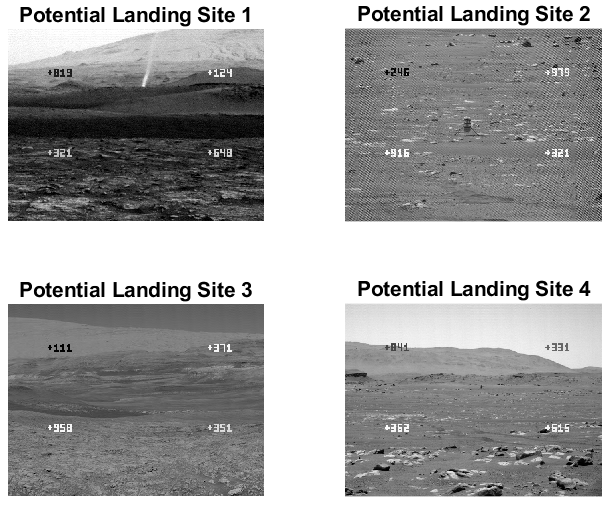
\includegraphics[width=10cm]{figures/p2-landingsites.png}
    \caption{All four sites recovered\label{fig:p2-landingsites}}
\end{figure}
\begin{table}[ht]
    \small
    \caption{Navigational Numbers For Each Site\label{tab:p2-landingsites}}
    \begin{tabularx}{\textwidth}{c| *{5}{Y} }
        Site   & Top Left & Top Right & Bottom Left & Bottom Right \\
        \hline
        Site 1 & 819      & 124       & 321         & 648          \\
        Site 2 & 246      & 979       & 916         & 321          \\
        Site 3 & 111      & 371       & 958         & 351          \\
        Site 4 & 841      & 331       & 362         & 615
    \end{tabularx}
\end{table}

It appears as though site 4 may be the ideal landing site, as it is the only
image showing a large landscape that is almost entirely flat except for the far
away mountains. Site 2 could possibly be a good site, however there is not a
large field of view in the image, leaving uncertainty about the surrounding
terrain. Sites 1 and 3 have large mountains and valleys, and are therefore
unsuitable for ensuring a safe landing.

\pagebreak
%--------------------------------------------------------------------------
%
% SECTION 3: IMPULSE ANALYSIS
%
%--------------------------------------------------------------------------
\section{Habitat Impulse Analysis}
With a landing site chosen, the base of operations has been set up. In order to
ensure safety of occupants, acoustic properties of rooms in the habitat must be
analysed. For this analyses, the team has recorded the impulse responses of
different rooms, and sent them back to the team at BASA headquarters. The
signal is in the form of a Frequency Division Multiplexed (FDM) data stream,
with all impulse responses and text describing locations within the same 0.5s
signal. In the case of the habitat's acoustic responses, all intended messages
are multiplexed to occupy 8kHz of bandwidth at differing sub-carrier
frequencies. To recover the messages, the command centre's hardware system
analyses the incoming spectrum, demultiplexes the signals, applies analogue
filtering and then the signals are sampled by an analogue to digital converter.
\subsection{Spectrum Analyser}
The Fourier transform of the signal is used to plot the magnitude spectrum in
MATLAB\@. This is done by first determining the time and frequency vectors for
the signal, knowing that incoming signal is sampled at \verb+fs=576+kHz:

\begin{minted}{matlab}
    Ts = 1/fs;                                                  % Sampling Period [s]
    t = 0:Ts:0.5; t(end) = [];                                  % Time vector
    f = linspace(-fs/2, fs/2, length(t)+1); f(end) = [];        % Frequency Vector
    MUXSIG = fft(muxSignal);                                    % Fourier Transform
\end{minted}

Plotting both the time and frequency domains in Fig.~\ref{fig:p3-multiplexed},
the signal is clearly composed of 6 multiplexed signals, as shown by the six
clear peaks in the frequency domain, mirrored in both the positive and negative
frequencies.

\begin{figure}[ht]
    \centering
    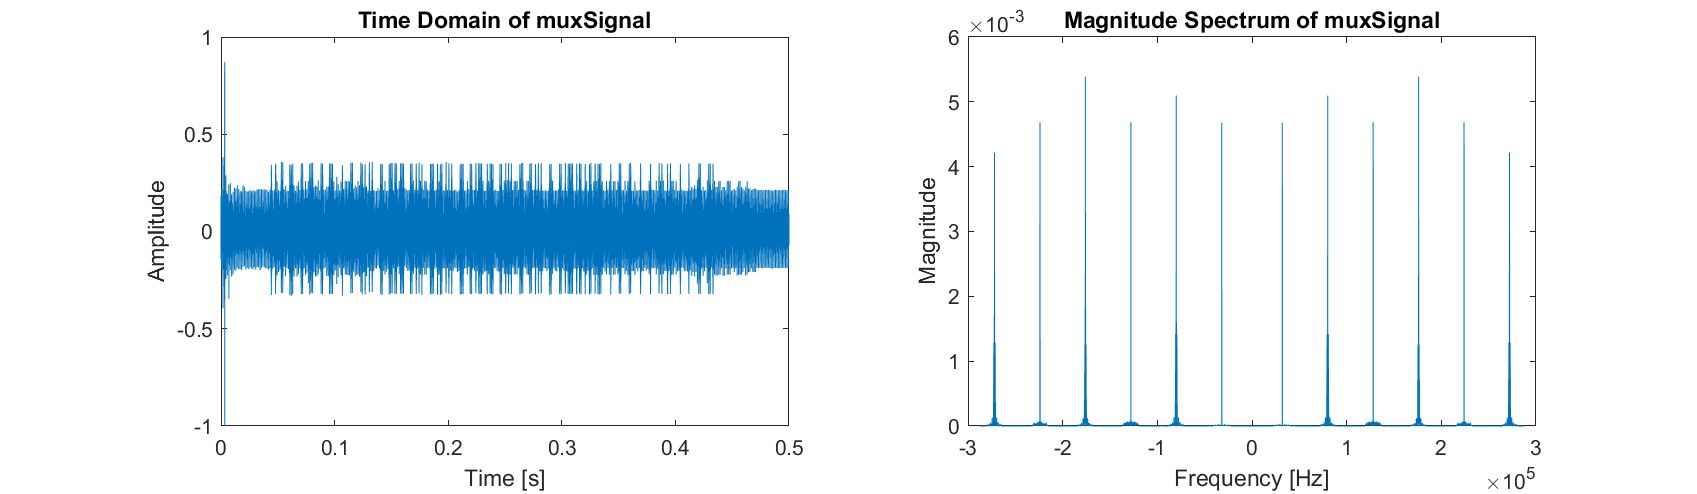
\includegraphics{figures/p3-multiplexed.png}
    \caption{Recieved Signal in Time and Frequency Domains\label{fig:p3-multiplexed}}
\end{figure}

\subsection{Demultiplexing}\label{sec:p3-demultiplexing}
The \verb+findpeaks+ MATLAB function was used to find the exact sub-carrier
frequencies efficiently and accurately. The magnitude and phase of those
frequency shifts was then determined, ensuring that demultiplexing can
accurately recover the signals despite any phase shift or magnitude distorsion.
\begin{minted}{matlab}
    MUXSIGshift = fftshift(MUXSIG);                             % Shift to correspond to f
    % Find 6 highest peaks (+ve frequencies)
    [~, fshift] = findpeaks(abs(MUXSIGshift(f>0)), f(f>0), 'NPeaks',6, 'SortStr','descend'); 
    fshift = sort(fshift);                                      % Sort in asc order
    fshift_indices = find(ismember(f, fshift));                 % Find indices within f
    Mag = abs(MUXSIGshift(fshift_indices));                     % Corresponding Magnitudes
    Phase = angle(MUXSIGshift(fshift_indices));                 % Corresponding Phase [rads]    
\end{minted}

The 6 signal streams were then recovered using a function provided by the team
at BASA, \verb+FDMDemux+. This function takes the signal, the frequency shifts,
and the corresponding magnitudes and phases, and returns a matrix containing
each individual demultiplexed stream:

\begin{minted}{matlab}
    xdm = FDMDemux(muxSignal, t, Mag, fshift, Phase);           % Demultiplex using known values
    XDM = fft(xdm, length(xdm), 2);                             % Row-wise FT
\end{minted}

Plotting the demultiplexed signals in Fig.~\ref{fig:p3-demultiplexed}, we can
see that there are 6 distinct signals, however the frequency domains clearly
show leftover noise from the demultiplexing process. Data within each stream
occupies 8kHz bandwidth, so the high-frequency noise will need to be filtered
to fully recover each signal. Since the streams have been demultiplexed, a
low-pass filter will be ideal for this process.
\begin{figure}[ht]
    \centering
    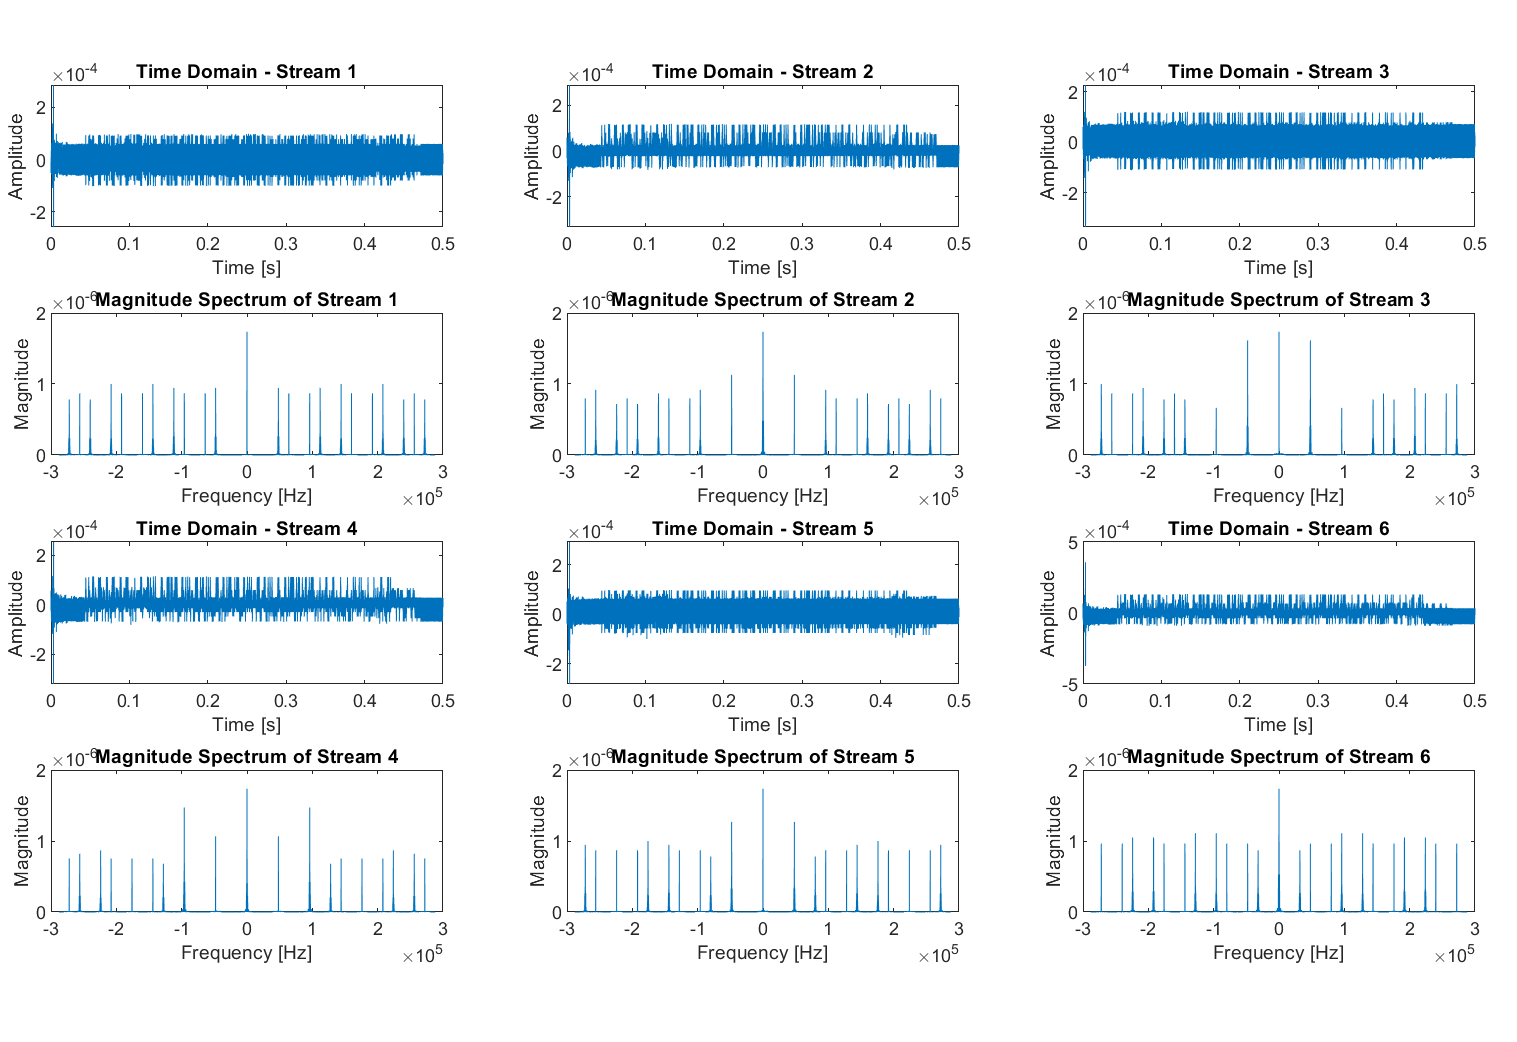
\includegraphics[width=\textwidth]{figures/p3-demultiplexed.png}
    \caption{Demultiplexed Data Streams in Time and Frequency Domains\label{fig:p3-demultiplexed}}
\end{figure}

\pagebreak
\subsection{Filtering}
BASA has provided four candidate filter circuits and their corresponding
transfer functions. The four transfer functions, as shown in MATLAB, are
depicted in Fig.~\ref{fig:p3-tfs}:

\begin{figure}[ht]
    \centering
    \begin{tabular}{cc}
        \verb+sys(1)+                                              & \verb+sys(3)+                                             \\
        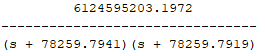
\includegraphics[width=0.28\textwidth]{figures/p3-tf1.png} & 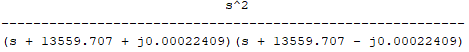
\includegraphics[width=0.5\textwidth]{figures/p3-tf3.png} \\
        \verb+sys(2)+                                              & \verb+sys(4)+                                             \\
        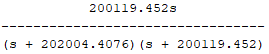
\includegraphics[width=0.28\textwidth]{figures/p3-tf2.png} & 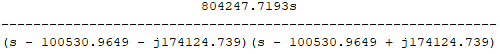
\includegraphics[width=0.5\textwidth]{figures/p3-tf4.png} \\
    \end{tabular}
    \caption{Transfer Functions of Candidate Circuits\label{fig:p3-tfs}}
\end{figure}

Knowing the properties of Laplace transforms, the poles of each system can
indicate important information regarding stability and impulse response. The
poles are represented in the denominator of each transfer function, so each was
analysed to determine possible suitability.

\begin{itemize}[noitemsep]
    \item[\textbf{sys(1):}] Real, negative poles. Indicates a stable system with exponential
        decaying impulse response.
    \item[\textbf{sys(2):}] Real, negative poles. Indicates a stable system. Magnitude of poles
        greater than system 1, so will likely have a quicker impulse decay comparatively.
    \item[\textbf{sys(3):}] Negative complex conjugate poles indicate sinusoidal components within
        the impulse response. Likely a stable system but oscillation may not be ideal.
    \item[\textbf{sys(4):}] Complex positive poles indicate an unstable system. Not fit for our purposes.
\end{itemize}

The systems were also visualised in MATLAB, analysing the poles and zeros,
impulse response (all except unstable system 4), and simulated frequency
response in both a bode plot and our frequencies of interest (see
Fig.~\ref{fig:p3-sys-analysis}).

\begin{figure}[ht]
    \centering
    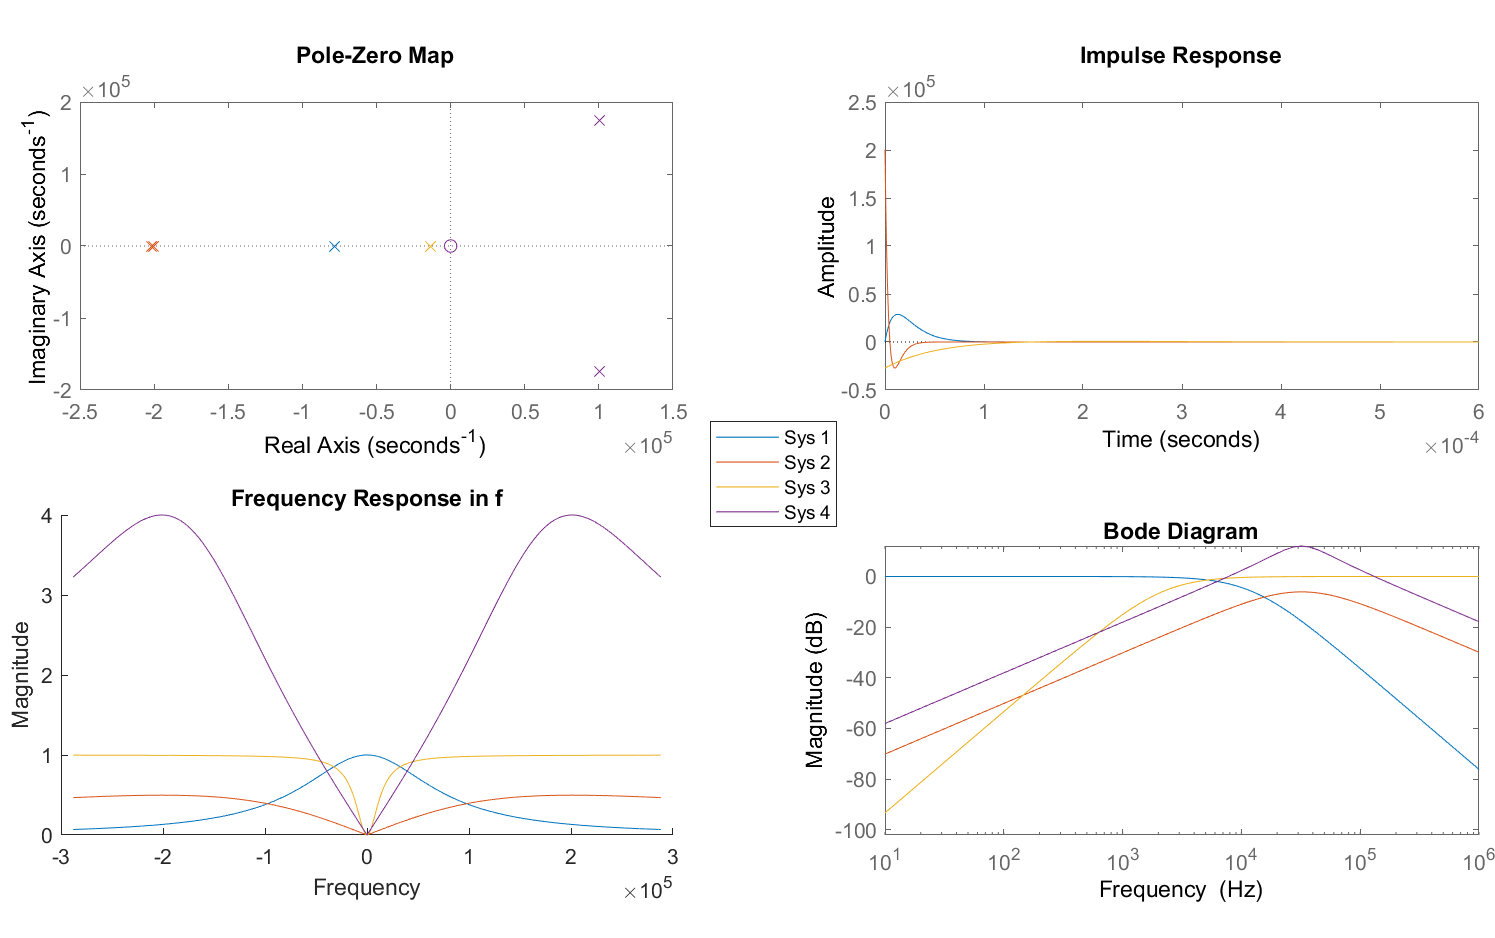
\includegraphics[width=14cm]{figures/p3-sys-analysis.png}
    \caption{System Analysis of Candidate Circuits\label{fig:p3-sys-analysis}}
\end{figure}

System 1 was chosen as the best candidate, as it has characteristics of a low
pass filter in the bode diagram. The impulse response rises and decays
exponentially without in a short period of time, without oscillatory behaviour.
Looking at the frequency response of the system, we can see that the the bode
diagram indicates less than 1.5dB attenuation throughout the 0-8kHz band,
before rolling off at 40dB per decade. This is the implication of using real
analogue filters; the roll off cannot be infinitely steep, so some amount of
noise will remain outside the desired band.

To apply the filter in MATLAB, the frequency response of system 1 was
multiplied by each stream in the frequency domain. To get this accurate
frequency response vector, first the impulse response is computed for \verb+t+,
which is the inverse laplace tranform of the systems transfer function in the
s-domain. The frequency response is then the fourier transform of this impulse
response. The frequency response could also be computed directly by
substituting $j\omega$ for $s$ in the transfer function.

\begin{minted}{matlab}
    syms s;                                                     % Define symbolic s
    [Num,Den] = tfdata(sys(1),'v');                             % Extract numerator and denominator
    sys1_TF = poly2sym(Num, s)/poly2sym(Den, s);                % Get symbolic transfer function
    sys1_IR = matlabFunction(ilaplace(sys1_TF));                % Usable function for impulse response
    impresp = sys1_IR(t);                                       % Discrete impulse response vector
    freqRes = fft(impresp);                                     % Discrete Frequency response
    MSG = zeros(size(XDM));                                     % Inilialise size For Performance
    for k = 1:size(XDM, 1)
        MSG(k, :) = freqRes .* XDM(k, :);                       % Apply the Transfer Function
    end
\end{minted}

The signals were then converted back to the time domain using an inverse
fourier transform. DC offset introduced by the filtering process was removed by
adjusting the mean of each signal to 0. Finally, streams were scaled to occupy
the amplitude range of $[-1, 1]$. Fig.~\ref{fig:p3-filteredstreams} shows the
resultant time and frequency domains of each stream after filtering, scaling,
and DC removal.

\begin{figure}[ht]
    \centering
    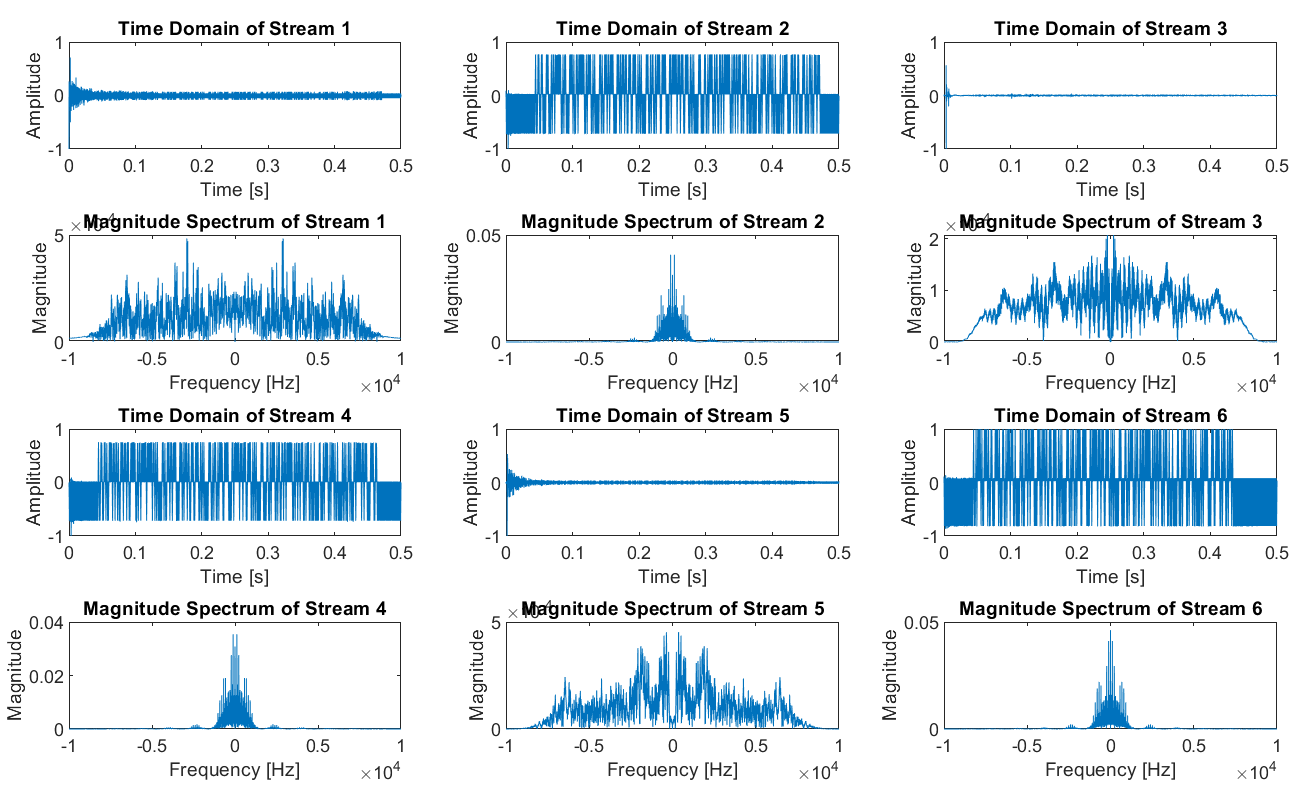
\includegraphics[width=0.9\textwidth]{figures/p3-filteredstreams.png}
    \caption{Filtered Data Streams in Time and Frequency Domains\label{fig:p3-filteredstreams}}
\end{figure}
\pagebreak
\subsection{Analogue to Digital Conversion}
Impulse response signals are sampled at 16kHz by a DAC\@. To simulate this
process, the matlab \verb+resample+ function can be used. The following code
resamples each of the impulse response signals (stream 1, 3, 5) to 16kHz:

\begin{minted}[]{matlab}
    FS_recov = 16e3;                                                % ADC sample rate [Fs]
    impulses_recov = resample(msg((1:2:end), :).', FS_recov, fs).'; % Resample each impulse response stream
\end{minted}

With impulse responses resampled, new time and frequency vectors conforming to
Nyquist sampling parameters were created to plot the digital signals in
Fig.~\ref{fig:p3-impulse-responses}. Text streams were decoded using the
supplied \verb+decoder+ function, displaying the room and astronaut who took
the measurements in the title of each corresponding plot.

\begin{figure}[ht]
    \centering
    \begin{subfigure}{0.5\textwidth}
        \centering
        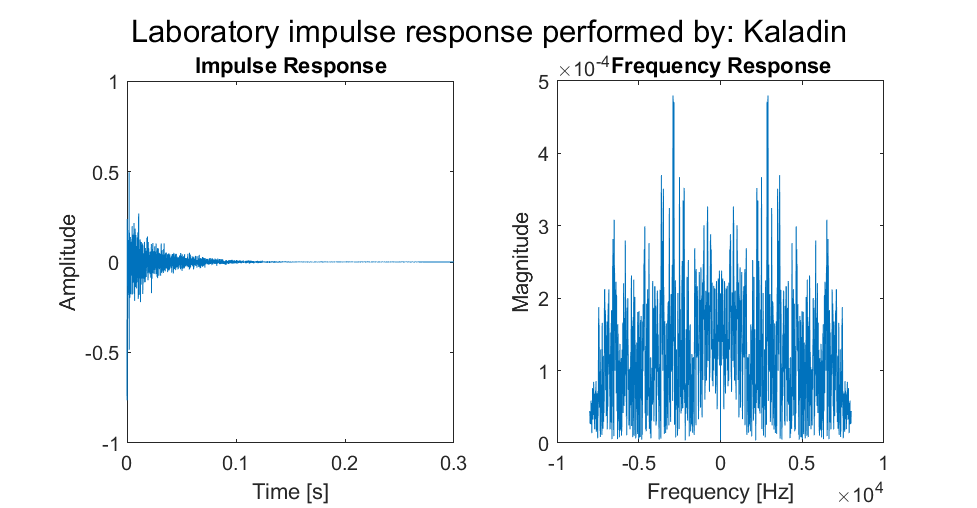
\includegraphics[width=\textwidth]{figures/p3-lab.png}
        \caption{Laboratory\label{fig:p3-lab}}
    \end{subfigure}%
    \begin{subfigure}{0.5\textwidth}
        \centering
        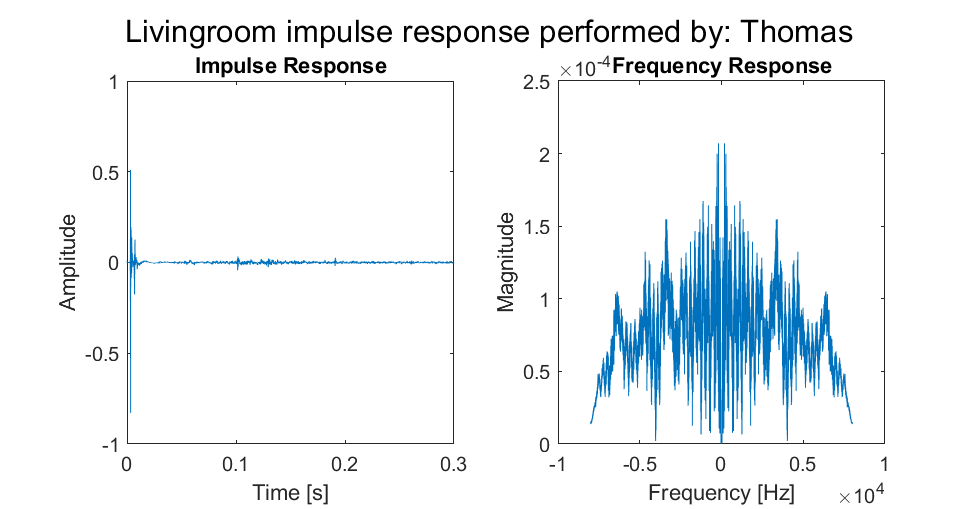
\includegraphics[width=\textwidth]{figures/p3-livingroom.png}
        \caption{Livingroom\label{fig:p3-livingroom}}
    \end{subfigure} \\
    \begin{subfigure}{\textwidth}
        \centering
        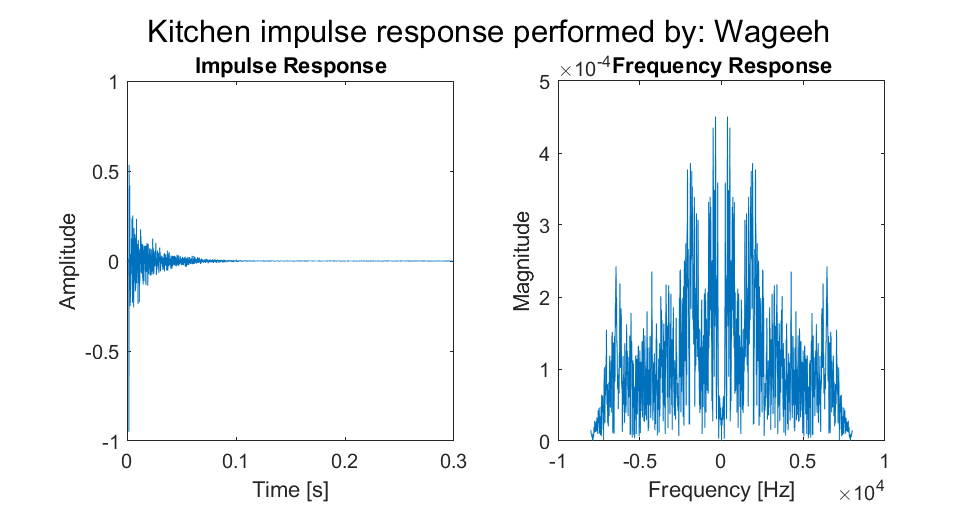
\includegraphics[width=0.5\textwidth]{figures/p3-kitchen.png}
        \caption{Kitchen\label{fig:p3-kitchen}}
    \end{subfigure}
    \caption{Received Impulse Responses\label{fig:p3-impulse-responses}}
\end{figure}

\pagebreak
\subsection{Practical Analysis}
Finally, to confirm that the impulse responses received are an accurate
representation of the locations they were gathered at, the impulse responses
were applied to recordings of our own voices. We can do this using a
convolution in the time domain, knowing that this represents multiplication in
the frequency domain:
\begin{equation*}
    f(x) * g(x) \xrightarrow{\mathscr{F}} F(f) \times G(f)
\end{equation*}
In MATLAB, the voice recording is read into a row vector, and first resampled
to match the sampling rate of the impulse responses. The resampled recording can then be
convolved with the impulse response of each room.

\begin{minted}[]{matlab}
    [voice, fs_voice] = audioread("voice.wav");
    % convert to row vector and only use one channel
    voice = voice(:, 1).';
    voice = resample(voice, FS_recov, fs_voice);                    % Resample voice to match impulse responses
    % apply the impulse response as a convolution in the time domain
    voiceTest = zeros([size(impulses_recov, 1) length(voice)]);     % Initialise size for performance
    for k=1:size(impulses_recov, 1)
        voiceTest(k, :) = conv(voice, impulses_recov(k, :), 'same');% 'same' ensures length is preserved
    end
\end{minted}

Comparing the original voice recording to the resultant signals in
Fig.~\ref{fig:p3-voicetest}, it can be seen that the original shape of the
waveform is preserved with minor variations. The resultant waveforms have
distinctly different sounds to them, as if the recording was made at the
location of the impulse responses. Specifically, when convolved with the
impulse responses of these rooms, there is a clear echo present in all three
results, with the most obvious being the living room impulse response.

\begin{figure}[ht]
    \centering
    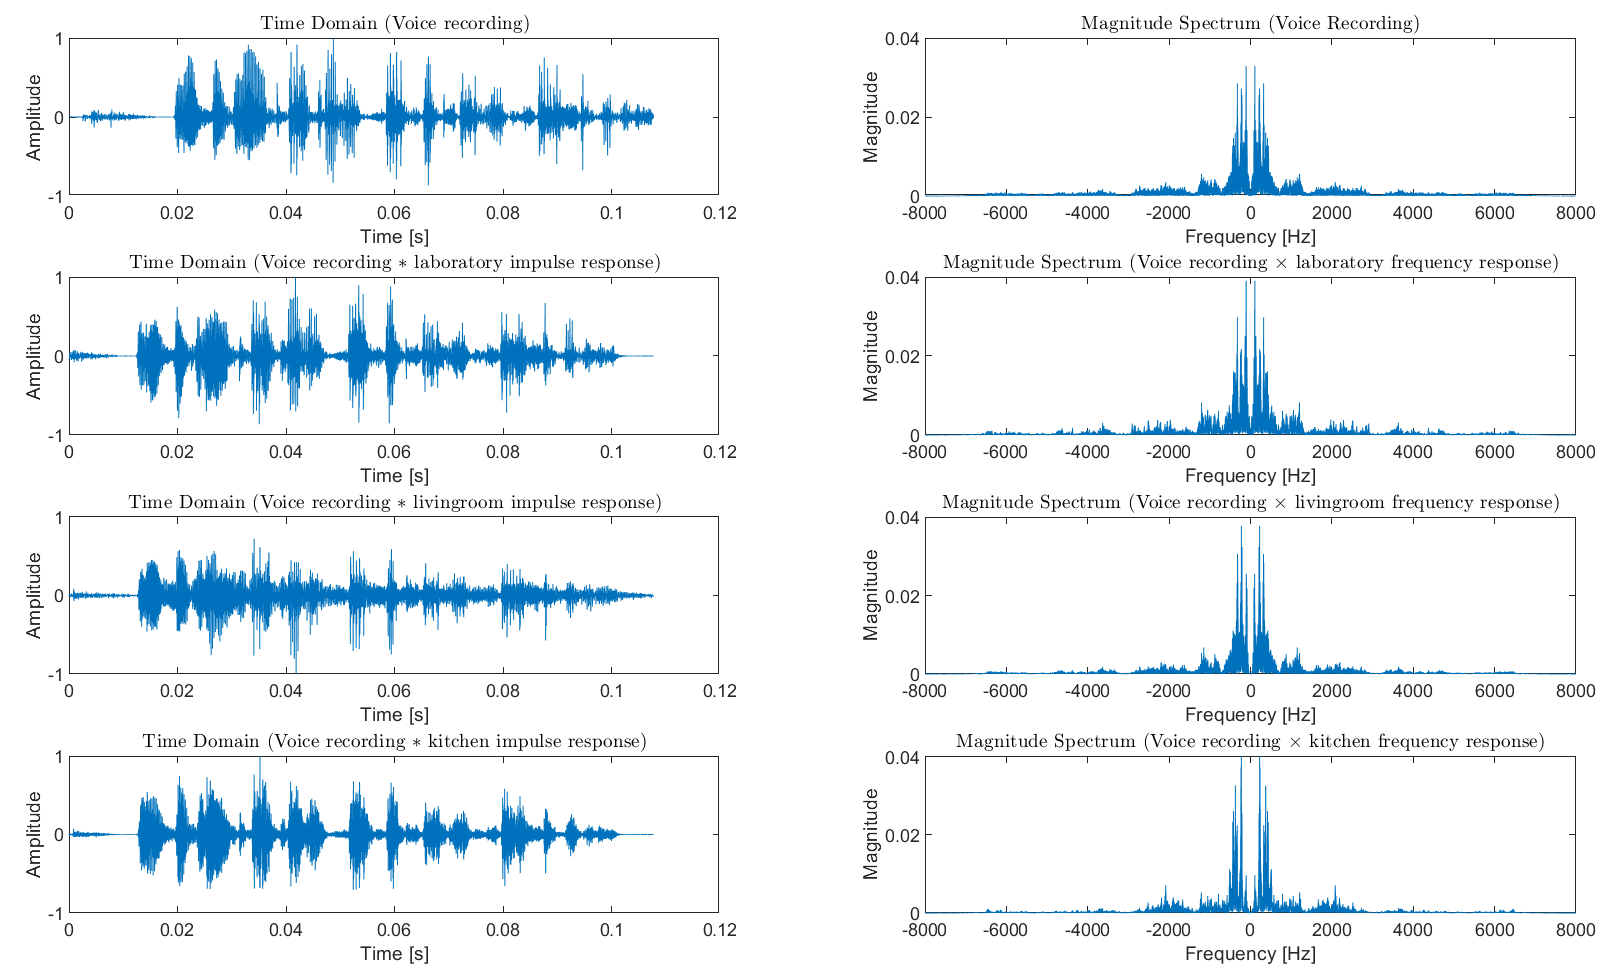
\includegraphics[width=\textwidth]{figures/p3-voicetest.png}
    \caption{Voice and Impulse Response Testing\label{fig:p3-voicetest}}
\end{figure}

\section{Reflection}
\pagebreak

\end{document}